% BEÁLLÍTÁSOK - JOBB NEM VÁLTOZTATNI
\documentclass[final]{ubb_dolgozat}

\usepackage{definitions}
\usepackage{comment}
% milyen nyelveken akarunk forráskódot megjeleníteni
\lstloadlanguages{Java,C++, html}
% más lehetőségek:
% C, Matlab, Mathematica, Octave, Pascal, Perl, Python
% SCilab, SQL, Haskell, Lisp, Lua, make, ML, PHP, Prolog
%
% a teljes lista a LISTINGS csomagban.


% ezt be lehet tenni MINDEGYIK megjelenítendő kód elé opcióként
\lstset{language=Java}


%%%%%%%%%%%%%%%%%%%%%%%%%%%%%%%%%%%%%%%%%%%%%%%
%%!!          EZT KELL VÁLTOZTATNI       !!%%%%
%%     A DOLGOZAT CÍMOLDALÁNAK ELEMEI        %%

%% MELYIK ÉVBEN ADJUK LE
\submityear{%
2018
}

\titleHU{%
Régiófejlesztésre és elszármazott szakemberek összekapcsolására kialakított közösségi háló
}

% Az alábbi sorokat ki kell tölteni!!

\titleEN{%
Social network for regional development and linking emigrated professionals 
}

\titleRO{%
Rețea de socializare pentru dezvoltarea regională și de a interconecta profesioniști emigrați
}

\author{%
Borsay Zsuzsanna
}

%%
\tutorHU{%
Csaba Sulyok,\newline doktorandusz
\newline dr. Simon Károly\newline egyetemi adjunktus
% a hozzátartozás akkor szükség, ha NEM BBTE-s a tanár
%{\large Babe\c{s}--Bolyai Tudományegyetem,\\
% Matematika és Informatika Kar}% ha különbözik, akkor fel kell tûntetni
}
%%
\tutorRO{%
Lector dr. Károly Simon\\
drd. Csaba Sulyok
% az egyetem akkor szükség, ha nem BBTE-s a tanás, a minta a BBTE-t
% tartalmazza
% {\large Universitatea Babe\c{s}--Bolyai,\\ % dacã diferã!!!
% Facultatea de Matematic\u{a} \c{s}i Informatic\u{a} }%
}
%%
\tutorEN{%
Assist prof. dr. Károly Simon\\
drd. Csaba Sulyok
% {\large Babe\c{s}--Bolyai University,\\
% Faculty of Mathematics and Informatics}
}


% 
%\includeonly{bevezet}


\begin{document}

%% ABSTRAKT
\begin{abstractEN} % ANGOL VÁLTOZAT

% a lenti részt értelemszerûen ki kell tölteni a dolgozat angol kivonatával.
% A BEGIN ... END között CSAK A SAJÁT SZÖVEG kell, hogy legyen.
% Az utolsó mondatot benne kell hagyni, mely által kijelentitek, hogy a munkátok SAJÁT.


{

	\vfill
  
  \center{
  
  {\huge EZ AZ OLDAL NEM RÉSZE A DOLGOZATNAK!}
	
	\vspace{0.5cm}
	
	{\Large Ezt az angol kivonatot külön lapra kell nyomtatni és alá kell írni!}
	
	\vspace{0.5cm}
	
	{\huge A DOLGOZATTAL EGYÜTT KELL BEADNI!}
  
  }
	
	\vfill

	Kötelező befejezés:
}
\vspace*{.5cm}

This work is the result of my own activity. I have neither given nor received unauthorized assistance on this work.

\end{abstractEN}

% ez a címoldal része
\maketitle

%% 

% a dolgozat tartalomjegyzéke -- ez automatikusan generálódik a STRUKTÚRA alapján.
{ \baselineskip 1ex
  \parskip 1ex
  \tableofcontents
}


%%%%%%%%%%%%%%%%%%%%%%%%%%%%%%%%%%%%%%%%%%%%%%%%%%%%%%%%%%%
%%%%%%%%%%         a dolgozat tartalma         %%%%%%%%%%%%

% ajánlott külön file-okba írni az egyes fejezeteket,
% ugyanis úgy jobban át lehet látni.


% a bevezetõ fejezet FILE-ja.
%!TEX root = minta_dolgozat.tex
%%%%%%%%%%%%%%%%%%%%%%%%%%%%%%%%%%%%%%%%%%%%%%%%%%%%%%%%%%%%%%%%%%%%%%%
\chapter*{\textcolor{red}{Bevezető}}
\markboth{Bevezető}{Bevezető}
\addcontentsline{toc}{chapter}{Bevezető}
%%%%%%%%%%%%%%%%%%%%%%%%%%%%%%%%%%%%%%%%%%%%%%%%%%%%%%%%%%%%%%%%%%%%%%%

Napjainkban azt tapasztaljuk, hogy nagyon sok Székelyföldön született szakember dönt a külföldre való kivándorlás mellett. Tanulmányaikat befejezve, a jobb élet reményében, vagy a kíváncsiság által hajtva külföldre mennek, ott vállalnak munkát és telepednek le, rövidebb vagy hosszabb időre. Az E-migrated alkalmazás inspirációjául szolgáló projekt, Csala Dénes SZÉKELYDATA című projektje, ezeket a szakembereket kutatja fel, Facebook adatbányászatot használva, és jeleníti meg őket egy világtérképen (\ref{fig:szekely_diaszpora}. ábra~\footnote{Kép forrása: \url{http://csaladenes.egologo.ro/wp-content/uploads/2015/08/szekely_diaszpora12.jpg}, utolsó megtekintés dátuma: 2018-03-07}). Célja az volt, hogy statisztikákat készítsen arról, hogy hol élnek és mivel foglalkoznak az otthonaikat elhagyó, külföldre vándorolt székelyek. 

Az E-migrated alkalmazás tekinthető a SZÉKELYDATA projekt dinamikus, kibővített változataként. A főoldalon levő világtérképen a csatlakozott szakemberek klaszterezett formában jelennek meg és dinamikusan szűrhetőek foglalkozás szerint. A felhasználók módosíthatják lakhelyüket, ezáltal a hozzájuk rendelt térképjelzők az új lakcím szerinti helyüket foglalják el, így naprakészen tartva a térképen  megjelenített statisztikákat. 

Az alkalmazás a Digitális Székelyföld\footnote{Forrás: \url{http://digitalisszekelyfold.ro/}} projekt része, amely  a székelyföldi IT Plus Cluster által indított régiófejlesztési kezdeményezés. Az E-migrated projekt célja egy olyan webes szoftverrendszer kialakítása, amely összekapcsolja a külföldön élő, dolgozó szakembereket és lehetővé teszi számukra a szakmai tapasztalatcserét, tudásmegosztást és az egymásnak való segítségnyújtást, kialakítva egy digitális polgárságot. Az alkalmazás felhasználói olyan külföldön vagy itthon élő, szakmájukban kiemelkedő teljesítményt nyújtó személyek, akik Székelyföldön születtek és szeretnének hozzájárulni szülőföldük technológiai és gazdasági fejlődéséhez. 

A dolgozat további része bemutatja a projekt működését, a felhasznált technológiákat, eszközöket és munkamódszereket.  \Aref{ch:projektrol}. fejezet részletezi az alkalmazás funkcionalitásait, a különböző komponensek közötti kommunikáció megvalósítását, valamint az alkalmazás adatmodelljét.  \Aref{ch:szerver}. és \aref{ch:kliens}. fejezetekben bemutatásra kerülnek a szerver illetve kliens oldali architektúrális megoldások, az implementáció során használt technológiák és eszközök. \Aref{ch:egyebb_eszkozok}. fejezet leírja a fejlesztés során alkalmazott munkamódszereket,  a folyamatos integráció megvalósításához használt technológiákat, a build és függőségkezelő eszközöket, az implementáció során használt fejlesztői környezeteket, valamint a kód minőségét ellenőrző statikus kódelemzőket és teszteket. \Aref{ch:mukodes}. fejezetben kerül sor az alkalmazás működésének szemléltetésére felhasználói szemszögből, különböző ábrák segítségével. Az utolsó fejezet felvet pár továbbfejlesztési lehetőséget és levonja a következtetéseket. 
\begin{figure}
  \centering
  \pgfimage[width=1\linewidth]{images/szekely_diaszpora}
  \caption{A külföldön élő székelyföldiek feltérképezése Facebook bányászattal történt.}
  \label{fig:szekely_diaszpora}
\end{figure}

A projekt tervezése és megvalósítása a Codespring mentroprogram\footnote{Forrás: \url{https://edu.codespring.ro/}, utolsó megtekintés dátuma: 2018-02-27} nyári gyakorlata során kezdődött. Az alkalmazás fejlesztését Tüzes-Bölöni Kincsővel együtt kezdtük el, lefektetve az alkalmazás alapjait. A nyár folyamán fokozatosan bővülő specifikáció alapján, egymás után születtek meg az alkalmazás funkcionalitásai. Az egyetemi félév kezdetével, a Csoportos projekt\footnote{Forrás: \url{https://www.cs.ubbcluj.ro/files/curricula/2016/syllabus/IM_sem5_MLM5012_hu_csatol_2016_1984.pdf}, utolsó megtekintés dátuma: 2018-03-16} nevű tantárgy keretein belül, a csapat további három taggal egészült ki, akik szintén hozzájárultak az alkalmazás bővítéséhez. 

A projekt létrejöttéért és a fejlesztés során nyújtott támogatásért köszönet illeti a Codespringet, a mentoraimat, dr. Simon Károly egyetemi adjunktust, Sulyok Csaba doktoranduszt és Szász István szoftverfejlesztőt. Köszönet Szilágyi Zoltán szofterfejlesztőnek a frontend kódbázis alapos átnézéséért és értékeléséért. Nem utolsó sorban pedig köszönet illeti a sok segítségért, támogatásért és biztatásért Tüzes-Bölöni Kincsőt, aki nélkül a projekt nem jöhetett volna létre. 

Az E-migrated alkalmazás bemutatásra került az V. Székelyföldi IT\&C és Innovációs Konferencián\footnote{Forrás: \url{http://www.itpluscluster.ro/hu/node/399}, utolsó megtekintés dátuma: 2018-02-27} és az Erdélyi Tudományos Diákköri Konferencián\footnote{Forrás: \url{https://www.etdk.kmdsz.ro/2018/index.php}, utolsó megtekintés dátuma: 2018-11-07}, ahol dicséretben részesült. Köszönet illeti a konferenciák szervezőit, valamint az aktív résztvevőket, akiknek megjegyzései, hozzászólásai hozzájárultak az alkalmazás funkcionalitásainak bővítéséhez. 




\chapter{Az E-migrated projekt}\label{ch:projektrol}

\begin{osszefoglal}
Az alkalmazás célja egy olyan felület kialakítása, amely összekapcsolja a külföldön élő, Székelyföldről elszármazott szakembereket, ezáltal lehetővé téve számukra a kölcsönös segítségnyújtást és tapasztalatcserét. A jelen fejezet ismerteti a felhasználók számára elérhető funkcionalitásokat, bemutatja a szerver és kliens, illetve a szerver és adatbázis közötti kommunikációt és szemlélteti az alkalmazás adatmodelljét.
\end{osszefoglal}

\section{A projekt funkcionalitásai}\label{sec:projektrol:funkcionalitasok}

Ez a fejezet az érthetőségre és átláthatóságra törekedve bemutatja az alkalmazás összes funkcionalitását, nem csak az szerző által fejlesztetteket. Azokat a funkcionalitásokat, amelyek implementálásánál nagyobb szerepem volt, a use-case diagrammokon dőlt betüvel és narancssárga színnel jelöltem (\ref{fig:vendeg_use_case}., \ref{fig:felhasznalo_user_case}. és \ref{fig:admin_use_case}. ábrák). 

\begin{figure}
  \centering
  \pgfimage[width=0.8\linewidth]{images/vendeg_use_case}
  \caption{A vendég (nem bejelentkezett) felhasználók számára elérhető funkcionalitások.}
  \label{fig:vendeg_use_case}
\end{figure}
Az alkalmazás főoldalán egy világtérkép  látható, amelyen kluszterezett formában vannak megjelenítve a már csatlakozott szakemberek. A vendégfelhasználók (nem regisztrált felhasználók) szűrhetik a felhasználókat foglalkozás szerint, de nem jeleníthetnek meg róluk semmilyen személyes információt (\ref{fig:vendeg_use_case}. ábra). Amennyiben szeretnék látni a rendszer felhasználóinak publikus adatait, de nincsen olyan ismerősük, akitől meghívót kérhetnének, meghívó igénylést küldhetnek az adminisztrátornak, csatolva az önéletrajzukat és egy rövid motivációs levelet, amelyben megindokolják, hogy miért szeretnének csatlakozni.

\begin{figure}
  \centering
  \pgfimage[width=1\linewidth]{images/felhasznalo_use_case}
  \caption{A bejelentkezett felhasználók számára elérhető funkcionalitások.}
  \label{fig:felhasznalo_user_case}
\end{figure}

Regisztráció után az előbb említett térképen, rákattintva a térképjelzőkre kilistázhatják az adott régióban élő felhasználókat, illetve a felhasználók nevére kattintva átnavigálhatnak az adott személy publikus profil oldalára, ahol bővebb információhoz juthatnak (\ref{fig:felhasznalo_user_case}. ábra). 

A bejelentkezett felhasználók meghívókat küldhetnek ismerőseiknek és megtekinthetik a régebben elküldött meghívóikat, illetve, hogy azok el vannak-e fogadva vagy még függőben állnak. Kezdetben minden felhasználó korlátozott számú meghívóval rendelkezik, ami arra ösztönzi őket, hogy gondolják meg jól, hogy kinek küldik el azokat.

Egy meghívót kapott személy kétféle regisztráció közül választhat, regisztrálhat szociális háló segítségével, amely egyszerű, nem igényli bonyolult formok kitöltését, hiszen a rendszer minden szükséges információt megkap az adott szociális hálótól. A későbbiekben a bejelentkezés is történhet az adott háló segítségével, így nincs szükség újabb felhasználónév és jelszó megjegyzésére sem. Az alkalmazás jelenleg a Facebookkal való regisztrációt és bejelentkezést támogatja. A másik lehetőség a hagyományos regisztráció, amely során egy regisztrációs formot kell kitölteni általános profiladatokkal (név, felhasználónév, jelszó, foglalkozás stb.). Ha valaki hagyományosan regisztrált, de szeretné összekapcsolni a Facebook fiókját a már meglévő profiljával, annak érdekében, hogy egyszerűbbé tegye a bejelentkezést, megteheti ezt regisztráció után is. 

Minden felhasználó módosíthatja a regisztráció során megadott adatait, illetve kiegészítheti ezeket például profilképpel és Markdown szintaxissal megadott önéletrajzzal. Bármilyen profilmodósítás során, illetve regisztrációkor a felhasználók elismerik, hogy olvasták és elfogadják az E-migrated alkalmazás adatvédelemre vonatkozó szabályzatát, amely megfelel az európai GDPR (General Data Protection Regulation) elveknek\footnote{\url{https://www.eugdpr.org/}}. A szabályzat leírja, hogy az alkalmazás hogyan kezeli, hogyan tárolja illetve mire használja a felhasználó által megadott személyes adatokat.

A rendszerhez való csatlakozás után a felhasználók bejegyzéseket hozhatnak létre, megtekinthetik és törölhetik az általuk létrehozott bejegyzéseket, és böngészhetik a mások által közzétetteket. 

Egy bejelentkezett felhasználó törölheti a fiókját, ha már nem szeretné tovább használni az alkalmazást. Törlés során két lehetőség közül választhat: szeretnék, hogy a fiókjuk törlése során törlődjenek az általuk létrehozott bejegyzések, vagy szeretnék, ha a bejegyzéseik megmaradnának, annak érdekében, hogy a többi felhasználó továbbra is láthassa, illetve visszakereshesse azokat. Ha a második opciót választják a profiljuk törlése után, az összes általuk írt bejegyzés hozzá lesz rendelve egy névtelen felhasználói fiókhoz.

A rendszer adminisztrátorai részére elérhető minden olyan funkcionalitás, ami egy átlagos felhasználó számára, viszont számukra a lista további funkcionalitásokkal bővül. Adminisztrátor nézetbe való váltás után lehetőségük van szerkeszteni a foglalkozásokat, újakat vezetni be a rendszerbe, illetve törölni egy már meglévőt, ha nincsen hozzá rendelve egyetlen szakember se. Az adminisztrátorok bírálják el a beérkező meghívó kéréseket, elfogadhatják, elutasíthatják illetve törölhetik ezeket, egy esetleges rövid személyes üzenet kíséretében, amelyet az illető személy egy automatikus üzenet törzsébe ágyazva kap majd meg. 

Az adminisztrátorok kilistázhatják az alkalmazás felhasználóit, kereshetnek köztük név szerint és indokolt esetben fel is függeszthetnek egy felhasználói fiókot (\ref{fig:admin_use_case}. ábra). A felfüggesztett személyek e-mailben kapnak értesítést, és számukra a bejelentkezés nem lehetséges egészen addig, amíg az adminisztrátor újra nem aktiválja a profiljukat. 

\begin{figure}
  \centering
  \pgfimage[width=0.95\linewidth]{images/admin_use_case}
  \caption{Az adminisztrátorok számára elérhető funkcionalitások.}
  \label{fig:admin_use_case}
\end{figure}

\section{Komponensek kommunikációjának megvalósítása}\label{sec:projektrol:kommunikacio}
Az alkalmazás legösszetettebb komponense, a szerver, Java programozási nyelvben íródott és szolgáltatásait a web-kliens számára REST (Representational State Transfer) \cite{REST} konvencióknak megfelelő endpointokon keresztül publikálja, melyek HTTP kérések által érhetőek el. 
\begin{figure}[!t]
  \centering
  \pgfimage[width=0.65\linewidth]{images/kommunikacio}
  \caption{Az alkalmazás legösszetettebb komponense, a szerver, Java programozási nyelvben íródott és szolgáltatásait a webkliens számára REST konvencióknak megfelelő endpointokon keresztül publikálja, melyek HTTP kérések által érhetőek el. A perzisztencia megvalósítására MySQL adatbázist használ, mellyel a Spring JPA segítségével kommunikál.}
  \label{fig:kommunikacio}
\end{figure}

A REST egy olyan architektúrális modell, amelyet az állapot nélküli, kliens-szerver kommunikáció megvalósítására terveztek. Az állapotmentességből kifolyólag a szerver nem tárol információt a kliensről, ezért minden hozzá érkező kérésnek tartalmaznia kell a kliens azonosításához szükséges adatokat. Az adatok és a hozzájuk tartozó műveletek erőforrásokként vannak publikálva a szerver által, amelyeket meghatározott URI-k azonosítanak. Az adatok kezelése és módosítása a POST, PUT és DELETE műveletek által, míg az adatok lekérése a GET művelet segítségével valósítható meg. A szabvány nem szögezi le a kérések illetve a válaszok formátumát, de a leggyakrabban használt formátum az XML és JSON \cite{REST}. Az E-migrated projekt esetében a kérések és válaszok küldése JSON formátumban történik.  

A perzisztencia megvalósítására MySQL adatbázist használ, mellyel a Spring keretrendszer által biztosított Java Persistence API (JPA) imlementációja segítségével kommunikál. A Spring JPA egy absztrakciós szintet képvisel a JPA fölött, a fejlesztőknek nem kell implementálniuk az adathozzáférést végző osztályokat, elegendő kiterjeszteniük a keretrendszer által biztosított interfészeket. 



\section{Adatmodell}\label{sec:projektrol:adatmodell}
\begin{figure}[!t]
  \centering
  \pgfimage[height=0.7\linewidth]{images/adatmodell}
  \caption{Az E-migrated alapvető entitásai egyszerű Java Bean-ek, melyek a BaseEntity ősosztályból származnak. Az alkalmazás központi egysége a User osztály\protect{,} mely a rendszer felhasználóit ábrázolja. Hozzá kötődő entitások az Address\protect{,} Profession\protect{,} CurrentUser\protect{,} RegistrationToken és FacebookAccount osztályok\protect{,} valamint a Role enum. A meghívó igényléseket pedig az InvitationRequest osztály ábrázolja.}
  \label{fig:adatmodell}
\end{figure}

Az E-migrated alkalmazáson belüli entitások Java Beanek, amelyek egyszerű getter és setter
metódusokat, valamint egy paraméter nélküli konstruktort tartalmaznak. Minden bean a \texttt{BaseEntity} ősosztály leszármazottja. A \texttt{BaseEntity} egyetlen attributúmmal rendelkezik, a UUID-val, amely egy egyedi, rendszer szintű azonosító és a relációs adatbázisban az entitásoknak megfelelő táblák elsődleges kulcsa. 

Az E-migrated alkalmazás központi entitása a \texttt{User} osztály,  melynek attribútumai közé tartozik a felhasználó neve, jelszava, email címe, profilképe, önéletrajza, az általa kiválasztott nyelv és egyébb, a felhasználóhoz tartozó információk. 



Minden felhasználó rendelkezik egy lakcímmel, amely az adatbázisban egy külön táblában van eltárolva és a User oszályhoz egy az egyhez kapcsolatforma segítségével van hozzárendelve, annak ellenére, hogy lakhatnak többen is ugyanazon a helyen, viszont azért, hogy ha valaki módosítani szeretné a lakcímét, ne módosuljon más személy lakhelye is, a csapat ezt a megközelítést választotta. Az \texttt{Address} osztály fontos szerepet játszik a felhasználók clusterezett megjelenítésében a főoldalon található térképen. A \texttt{lat} és \texttt{lng} adattagjai tárolják egy felhasználó címének földrajzi hosszúság és szélesség koordinátáit, amely alapján a térképen a felhasználók csoportosítva vannak. 

A felhasználók foglalkozása szintén egy külön tábla az adatbázisban, és a két entitás egy a többhöz kapcsolat segítségével van összekötve, hiszen egy szakma tartozhat több személyhez is. A \texttt{Profession} model osztály tartalmazza a hozzá tartozó felhasználók számát, illetve egy kulcs-érték párost, amelyben tárolva van a foglalkozás neve tetszőleges számú nyelven.

A \texttt{Post} osztály egy felhasználó által készített bejegyzést jelképez. Tartalmazza a címét, szövegét, feltöltési dátumát illetve a felhasználót, akihez tartozik az adott bejegyzés.

Az \texttt{InvitationRequest} entitás teszi lehetővé a meghívók igénylését a közösséghez való csatlakozás érdekében. Tartalmazza  a meghívót kérő személy email címét, rövid motivációs levelét, önéletrajzát illetve az igénylés dátumát. 

A meghíváson alapuló regisztráció megvalósítását a \texttt{RegistrationToken} osztály biztosítja, mely tartalmazza magát a tokent, a token lejárati idejét, az email címet amelyre küldték a meghívót, illetve tárolja a felhasználót, aki küldte a meghívót. 

A szerepkör alapú jogosultságkezelés a \texttt{Role} enum típus segítségével valósul meg, melynek értéke lehet \texttt{ROLE\_USER} és \texttt{ROLE\_ADMIN}. Minden felhasználó rendelkezik egy szerepkörrel, amely regisztrációkor automatikusan a \texttt{ROLE\_USER} értéket kapja. 



\chapter{\textcolor{red}{Szerver oldali technológiák}}\label{ch:szerver}

\begin{osszefoglal}
Az E-migrated alkalmazás szerver oldali komponensének alapja a Java programozási nyelv és a Spring keretrendszer. Ez a fejezet bemutatja a szerver architekturális megoldásait, leírja a különböző rétegeket, a szerver oldalon használt technológiákat,  a komponensek működését és egymással való kommunikációját. 
\end{osszefoglal}

\section{\textcolor{red}{Szerver oldali architekturális megoldások}}
\label{sec:szerverArch}

A szerver töbrétegű architekturára épül \cite{MultitierArchitecture}, melynek előnye, hogy a különböző funkciókat megvalósító rétegek egymástól elkülöníthetőek, ezáltal a tőlük függő komponensek módosítása nélkül is lecserélhetőek, illetve a további bővítés és tesztelhetőség is egyszerűen kivitelezhetővé válik. A szerver oldali komponens architekturája \aref{fig:ServerArchitecture}. ábrán látható módon van modularizálva. 
\begin{figure}
  \centering
  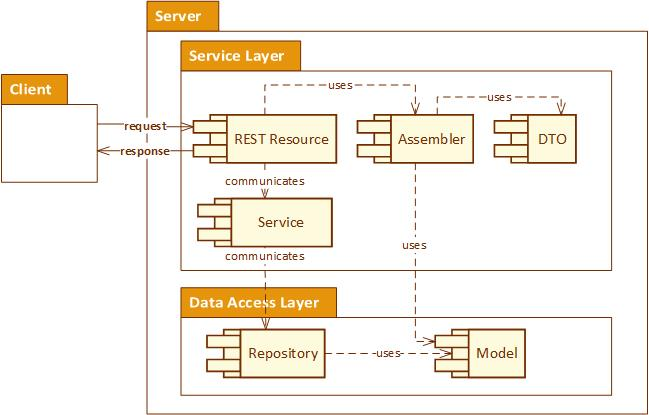
\includegraphics[width=1\linewidth]{images/ServerArchitecture}
  \caption{A szerver oldali komponens többrétegű architekturája  az \textit{adathozzáférési rétegből} (Model és Repository) valamint a \textit{szolgáltatási rétegből} (REST Resource, Assembler, DTO és Service) áll.}
  \label{fig:ServerArchitecture}
\end{figure}

Az \textit{adathozzáférési réteg} (data access layer) felelős az adatok perzisztenciájának megvalósításáért, valamint az alacsonyszintű adathozzáférés és az alkalmazás logika elkülönítéséért. Ehhez a réteghez tartoznak a \textit{Model} osztályok, amelyek az alkalmazás fő entitásai, és egyszerű POJO-k (Plain Old Java Object)~\cite{POJO} privát adattagokkal és publikus getter és setter metódusokkal, valamint a \textit{Model} objektumokat használó \textit{Repository} komponens. A \textit{Repository} komponens  által biztosított interfészek segítségével valósul meg a tulajdonképpeni adatkezelés, a DAO (Data Access Object)\cite{DAO} tervezési minta alkalmazásával. Az interfészek használatának előnye, hogy a réteg implementációja bármikor egyszerűen lecserélhető a felsőbb rétegek módosítása nélkül. 

A \textit{szolgáltatási réteg} tartalmazza az alkalmazás logikáját és meghatározza az adatokhoz való hozzáférési lehetőségeket. Az E-migrated projekt esetében ehhez a réteghez tartoznak a \textit{Service}, a \textit{Resource}, az \textit{Assembler}, valamint a \textit{DTO} komponensek. A \textit{Service} komponens használja az adathozzáférési réteg által publikált \textit{Repository} interfészeket és \textit{Model} osztályokat az adatkezeléssel kapcsolatos műveletek megvalósítása érdekében. Köztes szintet képvisel az adathozzáférés és az erőforráspuklikálás között. A szerver által biztosított REST erőforrások közzétételéért és a kliensnek küldött válaszok felépítéséért felelős \textit{Resource} komponens használja a  \textit{Service} és az \textit{Assembler} modulok által közzétett interfészeket, a HTTP protokkolon alapuló kommunikáció megvalósítása érdekében. Az \textit{Assembler} modul végzi az alkalmazás entitásai és a DTO-k közötti átalakítást, így biztosítva, hogy a kliens csak a számára szükséges adatokhoz férhessen hozzá. 



\begin{reviewed}
\section{Spring keretrendszer}
\label{subsec:Spring}

A Spring egy összefüggő infrastruktúrát biztosító Java keretrendszer.  Alappillérei az Inversion of Control (IoC) és a Dependency Injection (DI) technikák \cite{IoCDI}, amelyek kezelik és konfigurálják a komponenseket, menedzselik a példányokat és az ezek közötti függőségeket. Ezáltal a Spring leveszi a példányosítás és komplex konstruktormegírás terhét a fejlesztő válláról. Segítségével egy átlátható, moduláris alkalmazás hozható létre, mely klasszikus POJO-kra alapozva biztosítja az enterprise Java szolgáltatásait egy kompakt csomagolásban \cite{Spring}. 

A Spring keretrendszer moduljainak fő csoportja a Core Container~\cite{SpringCore}, amely többek között tartalmazza  a spring-core és spring-beans modulokat, amelyek biztosítják az IoC és DI funkciókat.

Az E-migrated egy Spring-Boot alapú alkalmazás, amely egy egyszerű módszer egy kezdetleges, futtatható Spring alkalmazás felépítésére. Erősségét és népszerűségét annak köszönheti, hogy a "convention over configuration" \cite{Convention} (konvenció konfigurálás fölött) elvet követve, a kezdeti beállításokat, konfigurációkat nem bízza a fejlesztőre, hanem alapértelmezett értéket ad ezeknek, ezáltal elősegítve az alkalmazás egy kezdeti, működő verziójának felépítését. Ez megkönnyíti a külső fejlesztőkkel való kollaborációt is, mert könnyen olvashatóvá teszi a kódot, és a konvenciók számukra is ismerősek lesznek. Természetesen ezek a beállítások a későbbiekben egyszerűen módosíthatóak.\cite{SpringBoot}
\section{Adathozzáférés és adattárolás}
\label{subsec:Adathozzáférés}
Az E-migrated alkalmazás szervere MySQL relációs adatbázist használ az adatok tárolására, amellyel a Spring Data JPA segítségével kommunikál. A Spring keretrendszer az adathozzáférési réteg implementálására egyszerű és kényelmes megoldásokat nyújt. Olyan Data Access Object (DAO) támogatást biztosít, amely által a különböző  perziszenciát biztosító technológiák egységesen és könnyen kezelhetőek (\ref{fig:SpringDataJPA}. ábra). Biztosít egy absztrakciós szintet a  JDBC (Java Database Connectivity) API-hoz, így megkíméli a fejlesztőket a bonyolult, adatbázis specifikus lekérdezések írásától, az alacsonyszíntű részletek implementálásától. Ezen felül biztosít egy egységes hibakezelési módszert, így nem kell külön ismerni a különböző adatbázis specifikus hibákat. 

A \texttt{@Repository} annotáció gondoskodik arról, hogy a komponens szkennelő megtalálja és konfigurálja az adott adathozzáférést biztosító osztályt, így nem szükséges XML állomány a konfigurációk megadására. Az E-migrated alkalmazás esetében is az annotációs megoldás használatos.

A Spring keretrendszer támogatja  a Java Persistence API (JPA) integrációját, amely egy absztrakciós szintet képez a JDBC felett és segítségével szabványosítható az Object Relational Mapping (ORM).  Az ORM célja, hogy megkönnyítse az objektum orientált programozási nyelvek és relációs adatbázisok közötti leképezést \cite{DataAccess}.

Minden Data Access Object-nek vagy adathozzáférést implementáló osztálynak szüksége van egy erőforrás hozzáférést biztosító objektumra, amely a \texttt{@PersistenceContext} annotáció segítségével injektálható be, és amely a META-INF mappában található \textit{persistence.xml} állományban levő konfigurációkkal szabható testre.


 \begin{figure}
  \centering
  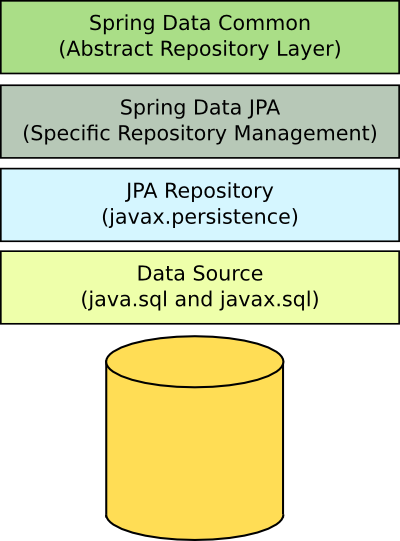
\includegraphics[height=0.5\linewidth]{images/SpringDataJPA}
  \caption{ \protect\footnotemark Spring Data keretrendszer család  lehetővé teszi az adat-hozzáférés egyszerű implementációját, a különböző adattárolási technológiák (pl. SQL és NoSQL adatbázisok) egységes módon való kezelését.}
  \label{fig:SpringDataJPA}
\end{figure}
\footnotetext{Kép forrása: \url{https://visola.github.io/2012/03/26/simple-spring-data-example/index.html}, utolsó megtekintés dátuma: 2018-04-19}

A Spring Data egy keretrendszer család, mely lehetővé teszi az adat-hozzáférés egyszerű implementációját, a különböző adattárolási technológiák (pl. SQL és NoSQL adatbázisok) egységes módon való kezelését. 
A Spring Data repository absztrakció fő interfésze a \texttt{Repository}. A \texttt{CrudRepository} ennek leszármazottja, és lehetővé teszi a CRUD (Create, Read, Update, Delete) műveletek egyszerű megadását. Nem szükséges implementálni a DAO osztályokat, elegendő csupán kiterjeszteni a Spring Data által biztosított interfészeket, és deklarálni a  számunkra szükséges metódusokat, a keretrendszer dinamikusan fel tudja építeni a megfelelő adaterélési parancsot \cite{DataJPA}. Például az  \texttt{InvitationRequestRepository} interfészben az \texttt{findByEmail} metódus, mely visszatéríti a paraméterként megadott e-mail címhez tartozó meghívó kérést, csak ki van jelentve, nincs implementálva, az implementációt a keretrendszer generálja, a betartott konvenciók alapján (\ref{fig:SpringData}. ábra). \texttt{create, read, update, delete} illetve más metódusokat, a keretrendszer a metódus nevéből és a programozó beállításaiból dinamukisan fel tudja építeni a megfelelő adatelérési parancsot \cite{DataJPA}.  
\begin{figure}
  \centering
  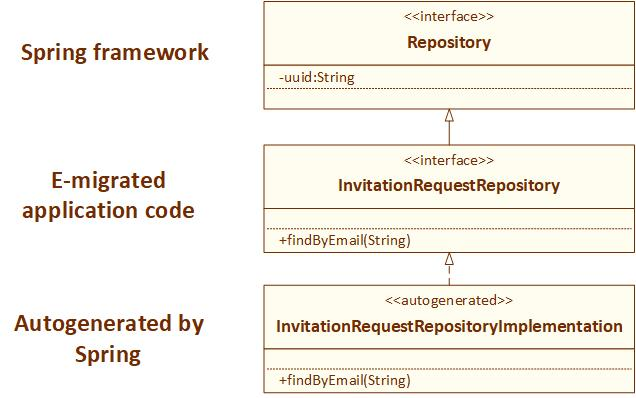
\includegraphics[width=0.7\linewidth]{images/SpringData}
  \caption{A Spring Data keretrendszer leveszi a fejlesztő válláról a DAO osztályok implementációját, elég kiterjeszteni a keretrendszer által biztosított interfészeket és a konvenciókat betartva deklarálni a metódusokat, a Spring a metódus nevéből automatikusan ki tudja generálni az implementációt.}
  \label{fig:SpringData}
\end{figure}

Lehetőség nyílik bonyolultabb lekérdezések egyszerű megadására is \texttt{NamedQuery}-k segítségével. A lekérdezéshez szükséges model osztály definíciója előtt a \texttt{@NamedQuery} annotáció segítségével felépíthető a lekérdezés, akár parametrizálva is. A lekérdezés törzsszövegében használt nyelvezet a  Java Persistence Query Language (JPQL), amelynek segítségével az entity modelre épített adatbázis lekérdezések írhatóak. A JPQL szintaxisa hasonlít az SQL nyelvezetére, de a Java környezetben levő entity osztályneveket használja a lekérdezések felépítésére, nem pedig az adatbázis oldalon levő tábla elnevezéseket.

\begin{listing}
  \inputminted{java}{progfiles/UserRepository.java}
  \caption{Bonyolult lekérdezés megvalósítása a Spring Data keretrendszer és NamedQuery-k segítségével.}
  \label{lst:userRepository}
\end{listing}


Példa erre többek között a \texttt{UserRepository} interfészben, az \ref{lst:userRepository}. kódrészletben található \texttt{findUsersLikeSearch()} metódus, amely a \texttt{search} paraméter által megadott szöveg alapján visszatéríti azokat a felhasználókat, akiknek a nevében megtalálható az adott szövegrész. Ez a metódus a többihez hasonlatosan nincsen implementálva, az adatbázis szintű lekérdezést a keretrendszer építi fel, a \texttt{User} model osztálydefiníciója előtt található \texttt{@NamedQuery} annotáció segítségével, amely a \ref{lst:namedQuery}. kódrészletben látható. A \texttt{@Param} annotáció köti össze a \texttt{@NamedQuery}-ben szereplő \texttt{:search} változót a metódus paraméterlistájában szereplő \texttt{search} paraméter értékével. Ennek segítségével bármilyen bonyolult lekérdezés egyszerűen megírható. 

\begin{listing}
  \inputminted[fontsize=\small]{java}{progfiles/UserNamedQuery.java}
  \caption{NamedQuery megadása a User bean osztálydefiníciója előtt, JPQL segítségével.}
  \label{lst:namedQuery}
\end{listing}

A Spring Data \texttt{PagingAndSortingRepository} interfésze olyan esetekben használható amikor nem szükséges, illetve nem kívánatos egyszerre az összes adatbázisban levő objektumot visszatéríteni, csupán azoknak egy részét, például az 10. objektumtól a 15. objektumig. A lapozás megvalósításához elegendő a \texttt{findAll()} metódus paraméterének átadni egy \texttt{PageRequest} objektumot, amelynek be van állítva, hogy hányadik oldalt térítse vissza, illetve, hogy egy oldalon hány objektum szerepeljen. Az almalmazáson belül a bejegyzések lapozása van megoldva a \texttt{PagingAndSortingRepository} segítségével.

Az E-migrated adathozzáférési rétegében minden az  \ref{sec:projektrol:adatmodell}. fejezetben említett model osztály  számára létezik egy neki megfelelő \texttt{Repository} interfész. Ezeken kívül még megtalálható a \texttt{UserConnectionRepository}, ami nem leszármazottja a \texttt{Repository} ősinterfésznek, natív implementációt tartalmaz, amire azért volt szükség, hogy a Facebook integráció esetében is biztosítani lehessen a meghíváson alapuló regisztrációt, mivel a Spring Social (lásd \ref{subsec:szocialisHalo}. fejezet) akkor is létrehoz egy bemenetet a \texttt{UserConnection} táblába, ha valaki illegálisan próbált bejelentkezni. Ezt a rekordot pedig törölni kell, hogy ne kapjon hibát az a személy, aki legálisan, meghívó által próbál regisztrálni az adott Facebook profillal, vagy épp hozzá akarja kötni ezt a Facebook profilt az E-migrated fiókjához.

\section{Üzleti logika réteg}
\label{subsec:szolgaltatas}
Az E-migrated alkalmazáson belül minden \texttt{Repository} osztályhoz tartozik egy \texttt{@Service} annotációval ellátott Service Spring Bean, amely injektálja a neki megfelelő \texttt{Repository} interfészt, ezáltal hivatkozhat annak metódusaira. Az alkalmazás szolgáltatási rétege a cserélhetőség érdekében egy interfészt publikál az API réteg számára, és ezeket az interfészeket implementálják a \texttt{ServiceImpl} osztályok. Ezáltal az API réteg egyszerűen injektálhatja ezeket az interfészeket, nem kell tudnia a háttérben levő implementációkról. 

A szolgáltatási réteg naplózza, burkolja és továbbítja a kivételeket a felsőbb rétegeknek. Minden szolgáltatási rétegbeli metódus hiba esetén dob egy \texttt{ServiceException}-t amit az API réteg kap el és kezel le.

A \texttt{UserService} osztály kezeli a felhasználókkal kapcsolatos műveleteket, mint például a regisztráció, bejelentkezés, jelszó és felhasználónév módosítás, Facebook által regisztrált felhasználók E-migrated fiókjának létrehozása, valamint visszatéríti a felhasználókat a bejövő paraméterek alapján. 

A \texttt{FacebookConnectionService} osztály hozzájárul a Facebook-kal való regisztráláshoz, illetve egy hagyományosan regisztrált felhasználó E-migrated fiókjának a Facebook profiljával való összekötéséhez (további információ a  \ref{subsec:szocialisHalo}. fejezetben).


\section{API réteg}
\label{subsec:API}

Mivel az API réteg felelős a klienssel való kommunikációért és ezt egy RESTful alkalmazás segítségével teszi meg, kézenfekvő volt használni a Spring által biztosított spring-web csomagot, amely segítségével egyszerűen implementálható egy RESTful alkalmazás. 
\end{reviewed}
\subsection{Spring Web modul}\label{subsubsec:SpringWeb}
A Spring Web modul lehetővé teszi egy Spring keretrendszerre épülő web-alkalmazás létrehozását bonyolult xml állományok nélkül. 

A Spring keretrendszerre épülő RESTful alkalmazások esetében a klienstől érkező kérések kezelését kontrollerek végzik. Egy kontroller a \texttt{@RestController}
annotáció segítségével adható meg. A HTTP kérések kezelőkhöz való rendelését a \texttt{@RequestMapping} annotáció biztosítja, mely meghatározza, hogy egy adott endpoint-ra érkező kérés esetén melyik metódus aktiválódjon.

Az E-migrated alkalmazás esetében a kontrollerek szerepét a \texttt{Resource} osztályok töltik be. Ezek az osztályok injektálják a számukra szükséges szolgáltatás-rétegbeli interfészeket, és ha szükséges továbbítják számukra az adatokat további feldolgozás érdekében.


\begin{reviewed}
\subsection{Data Transfer Object}
\label{subsubsec:DTO}
\begin{figure}[!b]
  \centering
  \pgfimage[width=0.9\linewidth]{images/Assembler}
  \caption{Az E-migrated alkalmazás a kliens és a szerver közötti adatmegosztásra DTO-kat használ. A DTO tervezési mintát alkalmazva minden Assembler egy ős Assemblerből származik, és minden Model, illetve DTO rendelkezik egy neki megfelelő Assemblerrel, mely az adott Modelt alakítja át DTO-vá illetve fordítva. A Resource osztályok ezeket az Assemblereket használva dolgozzák fel a beérkező adatatokat. }
  \label{fig:Assembler}
\end{figure}

A kliens és a szerver közötti adatmegosztás Data Transfer Objectek segítségével valósul meg. A DTO-k egyszerű POJO-k, melyek az attribútumaikat beállító és lekérdező getter és setter metódusokat tartalmaznak. A DTO tervezési mintának \cite{DTO} megfelelően minden Transfer Objectnek van egy megfelelő \texttt{Assembler} interfész, amelyek egy közös Assembler interfészből származnak, tehát kötelezően tartalmaznak legalább két metódust (\ref{fig:Assembler}. ábra). A metódusok deklarációjában levő M és D típusnevek egy-egy generikus típust jelölnek, melyet a specifikus \texttt{Assembler} interfészek határoznak meg attól függően, hogy melyik DTO-hoz tartoznak. Az említett metódusok közül az első egy adott \texttt{Model} objektumot alakít át egy neki megfelelő \texttt{DTO}-ra, a második pedig fordítva. 

Azokban az esetekben, ahol szükség volt a klienstől érkező adatok alapján egy \texttt{Model} objektum felépítésére és különböző alapértelmezett értékek beállítására az \texttt{Assembler} osztáyok tartalmaznak egy\texttt{ M create(D dto)} metódust is, amelyek visszatérítenek egy adott \texttt{Model} objektumot. Ilyen például a \texttt{RegistrationUserAssembler} is, ahol egy újonnan regisztrált felhasználónak be kell állítani, hogy kezdetben hány darab meghívóval rendelkezik, valamint az alapértelmezett nyelvet (magyar). Ezeket az alapértelmezett értékeket az \texttt{Assembler} osztály properties állományokból tölti be, hogy egyszerűen, a kód megértése nélkül lehessen változtatni az értéküket. A \texttt{@PropertySource("classpath:application.properties")} annotáció segítségével adható meg, hogy az osztály melyik állományból olvassa az értékeket, illetve az attribútumok deklarálásánál a \texttt{@Value("\${user.defaultNumberOfInvitations}")} annotáció határozza meg, hogy az adott állományból mely mező értékét vegye fel az annotált attribútum.

\section{Biztonsági megoldások}
\label{subsec:biztonsag}
A Spring Security összefogó biztonsági megoldásokat kínál vállalati Java alkalmazások számára. A két fő terület amit a Spring megcéloz a hitelesítés (authentication) és jogosultságellenőrzés (authorization) \cite{SpringSec}. 
A Spring Security testreszabása az alkalmazáson belül a  \texttt{SecurityConfig} osztályban található. Itt történik a felhasználók jelszavainak sózásához és hash-eléséhez szükséges kódolási algoritmus beállítása, amely ebben az esetben a Spring Security által biztosított, napjaink technológiáival visszafejthetetlennek vélt algoritmus, a \texttt{BCryptPasswordEncoder}. A Spring Security megkapja a felhasználó által beírt hitelesítési adatokat, ezeket kódolja, majd összehasonlítja az adatbázisban található hash-elt jelszóval, amennyiben a két jelszó megegyezik a hitelesítés sikeresen megtörtént, különben kivételt dob. 

A rendszeren belül használt \texttt{User} model osztály össze van kötve a Spring Security \texttt{User} osztályával, amely rendelkezik a felhasználónéven és jelszón kívül más attribútumokkal is, melyek további biztonsági ellenőrzéseket tesznek lehetővé, ilyen például az \texttt{accountNonLocked} adattagja. Az E-migrated alkalmazáson belül, ennek segítségével van megoldva, hogy a bejelentkezés sikertelen legyen, amennyiben a felhasználó fiókja fel van függesztve.

\begin{listing}[!b]
  \inputminted[fontsize=\small]{java}{progfiles/security.java}
  \caption{Egy \texttt{HttpSecurity} objektumon keresztül beállítható, hogy mi történjen, ha egy felhasználó nem megfelelő jogosultsággal próbál meg elérni egy erőforrást, illetve testreszabható, hogy mely útvonalak milyen jogosultsággal rendelkező személyek számára legyenek elérhetőek.}
  \label{lst:security}
\end{listing}

A klienstől érkező kérések jogosultságának elbírálását is a \texttt{SecurityConfig} osztályban levő beállítások határozzák meg. Itt van konfigurálva, hogy mi történjen, ha valaki nem megfelelő jogosultsággal próbál elérni egy erőforrást, illetve beállítható, hogy a különböző útvonalak, milyen szerepkörrel rendelkező felhasználók számára legyenek elérhetőek. Ebben a konfigurációs beanben vannak beállítva a sikeres, illetve sikertelen bejelentkezést kezelő útvonalak is (\ref{lst:security}. kódrészlet). 


Az E-migrated esetében az összes \texttt{/guest/**} formájú URL-re érkező kérés mindenkinek elérhető, viszont a \texttt{/user/**} és \texttt{/admin/**} URL-ek alatt levő erőforrásokat csak a megfelelő szerepkörrel rendelkező felhasználók érthetik el. Ugyanez a konvenció vonatkozik az \texttt{/api}-val kezdődő útvonalakra is.

\section{Szociális hálók integrálása}
\label{subsec:szocialisHalo}

Az E-migrated alkalmazásba való regisztráció lehetséges Facebook segítségével, de akár a későbbiekben is hozzákötheti egy felhasználó a Facebook profilját a már meglévő fiókjához. Ennek előnye, hogy nem kell regisztrációs form-ot kitölteni, illetve a bejelentkezés egyszerűbben történik. Az alkalmazás továbbfejlesztésként tervben áll a Google+ és Linkedln integráció is. 


A Spring Social \cite{SpringSocial} célja megkönnyíteni a fejlesztők számára a szociális hálók integrálását a Spring keretrendszerre épülő alkalmazásokba. A Spring Social egy adott felhasználó személyében küld kéréseket a szolgáltató API-jához. A bejelentkezés során a felhasználó a szolgáltató bejelentkezési oldalára lesz átirányítva ahonnan kap egy access tokent. Ez az access token regisztrációkor elmentődik az adatbázisba, tehát az E-migrated szervere ellenőrizni tudja, hogy regisztrált felhasználóról van-e szó. Amennyiben igen, visszatérít neki egy általa generált tokent (az E-migrated szerver esetében a felhasználó nevéből és Facebook ID-jából álló stringet) és ezt követően a felhasználó használhatja az E-migrated szolgáltatásait. 

Azért, hogy az alkalmazásba való regisztráció Facebook-os regisztráció esetében is meghívóhoz legyen kötve, szükséges volt kihasználni a Spring Social rugalmasságát és konfigurálhatóságát. Ennek érdekében a regisztráció során a
 \texttt{/signin/szolgáltató} útvonalra küldött POST kérés különböző rejtett mezőket tartalmaz. Ezekben a rejtett mezőkben kapja meg a szerver többek között a regisztrációs tokent, az email címet amelyre a meghívó volt küldve, illetve annak a személynek az azonosítóját, aki küldte a meghívót. Ezek a rejtett mezők a továbbiakban szesszió hatókörű kérés paraméterekként lesznek továbbítva egészen addig, amíg a szolgáltatótól kapott válasz meg nem érkezik. A válasz érkezése után, a rendszer a kapott válasz és a paraméterek alapján eldönti, hogy sikeres a belépés vagy a regisztráció, vagy nem, illetve ellenőrzi, hogy fel van-e függesztve a felhasználó fiókja. 

A Spring Social konfigurálása a \texttt{SocialConfig} konfigurációs bean-ben történik a csapat által írt adapterek és interceptorok beállításával. 

\section{E-mail küldő mechanizmus}
\label{subsec:e-mail}

Az E-migrated alkalmazás használata során több alkalommal is szükség van e-mail küldésére: meghívó küldése, értesítők kiküldése a profil felfüggesztése illettve újraaktiválása után.

A \texttt{MailSender} a Spring keretrendszer által biztosított fő interfész e-mailek kezelésére. Nagyon sok e-mailküldő rendszer esetében használható egyszerűsége miatt \cite{MailSender}. 

A \texttt{JavaMailSender} interfész a \texttt{MailSender} leszármazottja és ez már lehetőséget nyújt MIME típusú üzenetek küldésére is, általában a \texttt{MimeMessageHelper}-rel együtt használják, amely támogatja különböző csatolmányok (képek, dokumentumok, HTML oldalak) hozzáfűzését a levélhez \cite{JavaMail}. A referencia-implementációja a \texttt{JavaMailSenderImpl} osztály. 

A fejlesztőnek nem kell foglalkozni a Session konfigurálásával sem, a \texttt{JavaMailSender} gondoskodik erről is. Ezen felül biztosít egy kivétel hierarchiát is, melyek mind a \texttt{MailException} leszármozottjai. 

\begin{listing}
  \inputminted[fontsize=\small]{java}{progfiles/SendEmail.java}
  \caption{E-mail küldése a JavaMailSender interfész segítségével.}
  \label{lst:sendEmail}
\end{listing}

Az üzenet felépítése és küldése (\ref{lst:sendEmail}. kódrészlet) során egy \texttt{JavaMailSender} objektum \texttt{createMimeMessage()} metódusa által visszatérített \texttt{MimeMessage} megkapja az e-mail elküldéséhez szükséges adatokat, majd a \texttt{send()} metódus elküldi az üzenetet. 

Az E-migrated alkalmazás esetében a különböző e-mailek felépítése és elküldése, a \texttt{util} modulon belül levő \texttt{MailSenderBean} osztályban történik. Az e-mail küldéshez szükséges konfigurációs beállítások pedig a \texttt{conf} modulon belül a \texttt{MailSender} konfigurációs osztályban találhatóak meg. Ezeket az értékeket a rendszer egy \texttt{mail.properties} állományból olvassa be a \ref{subsubsec:DTO} fejezetben említett módon. Ebben az állományban található meg többek között az e-mailszerver elérési útvonala és azon belül az alkalmazásnak lefoglalt felhasználónév és jelszó.

A dinamikusan felépített e-mailek renderelése Freemarker templatek alapján történik a Spring Web MVC (Model View Controller) segítségével.
\end{reviewed}


\section{\textcolor{red}{Hibakezelés}}
\label{sec:hibakezeles}
A kivételkezelés az alkalmazáson belül rétegenként egységesen történik, melynek lényege, hogy az alsóbb rétegek naplózzák és burkolják a kivételeket, majd így továbbítják a felsőbb rétegeknek. Az adathozzáférési réteg által dobott kivételeket a szolgáltatási réteg kapja el, és burkolva továbbítja az API rétegnek. Az API réteg kezeli, és HTTP státusz kóddal kiegészítve továbbítja a kliens részére. Ennek előnye, hogy a rétegek egymástól függetlenné válnak, bármikor egyszerűen lecserélhetőek, és a felfele propagáló hibákból a kliens csak annyit lát, amennyire szüksége van, az implementációs részletek rejtve maradnak. 

A Spring Data Access modul segítségével az adathozzáférési réteg által dobott kivételek kezelése egységesen valósítható meg. A keretrendszer naplózza és \texttt{DataAccessException} objektumokba burkolja az ORM illetve a JDBC által dobott specifikus kivételeket. Ezeket a kivételeket a szolgáltatási réteg elkapja és kezeli, majd \texttt{ServiceException}-ökbe burkolva továbbítja az API rétegnek. A szolgáltatási rétegben fellépő hibák szintén \texttt{ServiceException}-ként lesznek továbbítva a felsőbb komponensnek. 

Az API réteg kommunikál a klienssel, tehát felelős a hibák megfelelő közvetítéséért is. Mivel a szerver a REST princípiumoknak megfelelő JSON formátumú üzenetek segítségével kommunikál a klienssel, hiba fellépése esetén is elvárt, hogy JSON formátumú választ küldjön. Ezért szükséges volt egy egységes hibakezelési módszer bevezetése, amely elkapja és a kliens számára megfelelő formára mappeli az API rétegben fellépő kivételeket.

A REST API kéréseket kezelő, \texttt{Resource} osztályok által dobott \texttt{ApiException}-öket, az \texttt{ErrorControllerAdvice} metódusai elkapják és a kivétel típusának megfelelő \texttt{ErrorMessageDTO}-t felépítve és beállítva a hozzáillő HTTP státuszkódot, JSON formátumú választ küldenek a kliensnek. \Aref{lst:apiException}. kódrészletben látható, ahogy a beérkező meghívó igényléseket kezelő metódus \texttt{ApiException}-t dob, ha a csatolt önéletrajz nem PDF formátumba volt feltöltve, illetve abban az esetben is, ha az e-mail küldése során kivétel lépett fel. Egy \texttt{ErrorMessageDTO} tartalmazza az üzenet szövegét egy string típusú kulcs formájában, amelyet a kliens oldali fordító értelmez és a megfelelő nyelven jelenít meg.
\begin{listing}
  \inputminted[fontsize=\small]{java}{progfiles/ApiException.java}
  \caption{A beérkező meghívó igényléseket kezelő metódus \texttt{ApiException}-t dob, ha a csatolt önéletrajz nem PDF formátumba volt feltöltve, illetve abban az esetben is, ha az e-mail küldése során kivétel lépett fel. Ezeket a kivételeket az \texttt{ErrorControllerAdvice} kapja el, mappeli és megfelelő formában továbbítja a kliens számára. }
  \label{lst:apiException}
\end{listing}

Az \texttt{ErrorControllerAdvice} egy Java Bean, amely a \texttt{@ControllerAdvice} annotációval van ellátva, ezáltal figyeli és elkapja a \texttt{@RestController}-ek által dobott kivételeket. Egy figyelni kívánt kivételt a kezelő metódus előtt a  \texttt{@ExceptionHandler} annotáció segítségével vezethetünk be (\ref{lst:errorControllerAdvice}. kódrészlet). Ez a megoldás lehetővé teszi az összes API rétegben fellépő hiba egyszerű és egységes mappalését. A specifikus hibákon kívül mappelve van az ős \texttt{Exception} osztály is, így biztosítva, hogy bármilyen váratlan hibára megfelelően reagáljon a szerver. Mivel a kivételeket a kliens \texttt{ErrorMessageDTO}-k formájában kapja meg, az implementációs részletek rejtve maradnak, viszont a számára fontos információ megjelenítésre kerül.  
\begin{listing}
  \inputminted[fontsize=\small]{java}{progfiles/ErrorControllerAdvice.java}
  \caption{Az \texttt{ErrorControllerAdvice} figyeli és elkapja a \texttt{@RestController}-ek által dobott kivételeket. Egy figyelni kívánt kivételt a kezelő metódus előtt a  \texttt{@ExceptionHandler} annotáció segítségével vezethetünk be. }
  \label{lst:errorControllerAdvice}
\end{listing}

A Spring Security a jogosultságellenőrzés során fellépő kivételeket statikus hibaoldal visszaküldésével kezeli, amely nem megengedhető egy olyan szerver számára, amely a REST princípiumokat betartva kommunikál a klienssel, így szükséges volt a keretrendszer által kínált hibakezelési módot testreszabni. Ez többek között a \texttt{SecurityConfig} osztályban valósul meg, ahol egy \texttt{HttpSecurity} objektumon keresztül beállítható, hogy minden hibás jogosultásg esetén a kérés legyen átirányítva az \texttt{/api/accessDenied} endpointra, amelyet az \texttt{AccessDeniedHandler} REST kontroller kezel és megfelelő formában közvetít a kliensnek.

A rétegspecifikus kivételek bevezetése lehetővé teszi a különböző rétegek egymástól független módon való lecserélését, tesztelhetőbbé és átláthatóbbá téve a kódot. Az API rétegben megvalósított hibakezelés biztosítja, hogy a klienstől érkező kérések során fellépő kivételek egységesen, JSON formátumú válaszok küldésével legyenek kezelve. 

\chapter{\textcolor{red}{Kliens oldali technológiák}}\label{ch:kliens}

\begin{osszefoglal}Az alkalmazás kliens oldali része egy single-page application (egyoldalas alkalmazás) \cite{SPA}, amelynek fejlesztése az AngularJS keretrendszer segítségével történt. A keretrendszer és az UI-Router által biztosított direktívák teszik lehetővé az alkalmazás különböző nézeteinek dinamikus felépítését, illetve a nézetek közötti egyszerű váltást, navigálást. A különböző nézetek elrendezése és megjelenítése az \texttt{index.html}-en, valamint a responsive design kialakitása a Bootstrap keretrendszer segítségével történik \cite{Bootstrap}.
\end{osszefoglal}

\section{\textcolor{red}{Kliens oldali architekturális megoldások}}
Az E-migrated alkalmazás kliens oldali MVC-t (Model-View-Controller) alkalmaz \cite{WebMVC}, ezáltal elkülönítve a nézetet az adatoktól és a vezérléstől. A kliens oldali MVC esetében a szerver csak statikus erőforrásként szolgál, nem teljesen felépített nézeteket küld vissza, csupán az ezek rendereléséhez szükséges adatokat szolgáltatja REST erőforrások formájában. A kliens oldal felelős ezek feldolgozásáért és megfelelő megjelenítéséért a kapott adatok és a meglévő sablonok alapján.
Az alkalmazás kliens oldalának architekturális megoldásai \aref{fig:ClientArchitecture} ábrán lathatóak. 

\begin{figure}
  \centering
  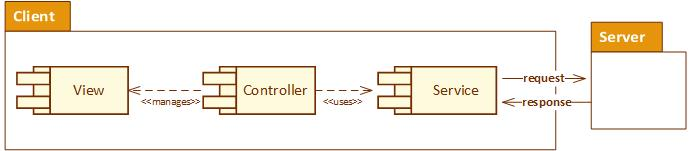
\includegraphics[width=0.9\linewidth]{images/ClientArchitecture}
  \caption{Az alkalmazás megjelenítési rétegét a kliens oldali komponens képviseli, a \textit{View}, \textit{Controller} és \textit{Service} modulok által. }
  \label{fig:ClientArchitecture}
\end{figure}

A \texttt{View} réteg biztosítja az alkalmazás felhasználói felületének megjelenítését. A felhasználók ezzel a réteggel lépnek direkt kapcsolatba, mely interakciókat a \texttt{Controller} észleli és irányítja. A \texttt{Controller} továbbítja a klienstől érkező kéréseket a service-eknek és a tőlük érkező válaszok alapján frissíti a nézetet. A \texttt{Service} réteg kommunikál a szerver API rétegével, JSON formátumú aszinkron kéréseket küldve és a válasz érkezése után továbbítja azokat a kontrollereknek. 

A webes komponens struktúrája az átláthatóság és az egyszerű bővíthetőség érdekében több, egymástól elkülönített részből épül fel, melyek a következők: \textit{services}, \textit{controllers}, \textit{directives} és \textit{config}. Az első kettő értelemszerűen a \texttt{Service} és a \texttt{Controller} rétegeket foglalja magába, míg a \textit{directives} modul tartalmazza a csapat által megírt direktívákat, amelyek hozzájárulnak a bonyolult nézetek egyszerűbb kezeléséhez és megjelenítéséhez. A \textit{config} modulban találhatóak a különböző konfigurációs beállítások, többek között itt történik a kontrollerek nézetekhez való hozzárendelése. 

\section{\textcolor{red}{AngularJS}}
\label{sec:angularjs}
Az AngularJS egy olyan JavaScript alapú, nyílt forráskódú keretrendszer, amely lehetővé teszi a kliens oldali MVC megvalósítását, illetve single-page alkalmazások egyszerű fejlesztését. Kiegészíti a HTML nyelvet különböző direktívákkal, így biztosítva a dinamikus nézetek létrehozását és a kétoldali adatkötést (two way data binding) \cite{AngularJS}.

A kétoldali adatkötés teszi lehetővé a nézetek automatikus frissítését, amennyiben a hozzárendelt modell objektum értéke változik, illetve a modell frissítését, ha a nézeten történik változás, ezáltal megszabadítva a fejlesztőket a DOM elemek kezelésétől és az ehhez tartozó kódok implementálásától. Az AngularJS modell objektumai egyszerű JavaScript objektumok.

A keretrendszer által biztosított Dependency Injection minta lehetővé teszi a komponensek számára a külső függőségeik használatát anélkül, hogy ismerniük kellene  a háttérben levő implementációt, ezáltal tesztelhetőbbé és átláthatóbbá téve a kódot. A keretrendszer injektálja és példányosítja is az adott függőséget, így nincs szükség bonyolult konstruktorhívásra.     

A DOM elemek viselkedésének meghatározása kontrollerek segítségével történik, ezáltal elválasztva a nézetet a vezérléstől, és így átláthatóbb, könnyebben tesztelhető alkalmazás-struktúrát hozva létre. A kontroller felelős a kliens interakcióinak figyeléséért és az ezekre való megfelelő viselkedés aktiválásáért. 



A keretrendszer lehetőséget nyújt új direktívák deklarálására is, amelyek segítségével alkalmazás specifikus, újrafelhasználható DOM elemek vezethetőek be a HTML nyelvbe. 


\section{\textcolor{red}{Web Controller}}
\label{sec:webController}
A Web Controller a kliens oldali MVC üzleti logika részét képezi. Felelős a nézetek inicializásáért, azok frissítéséért, illetve a service rétegektől érkező adatok megfelelő megjelenítéséért. 

Minden nézethez hozzárendelhető egy vagy több vezérlő, amelyeket az \texttt{ng-controller} direktívák segítségével vagy az \texttt{app.config} állományban állíthatunk be. A kontroller létrejövetelekor hozzárendelődik a DOM-hoz és egy \texttt{\$scope} objektumon keresztül hozzáférést kap a nézet elemeihez, amelyeket ezáltal irányíthat és módosíthatja tulajdonságaikat. 

A nézet inicializálása az \texttt{ng-init} direktívának megadott metódus aktiválása által történik, automatikusan. Minden a nézetben használni kívánt metódust hozzá kell rendelni a vezérlő \texttt{\$scope}  objektumához. Ez teszi lehetővé, hogy a kontroller különböző események hatására megfelelő viselkedést biztosíthasson. Ilyen esemény lehet például egy gombra való kattintás, amely során a gomb \texttt{ng-click} direktívájának értékeként megadott metódus aktiválódik. \Aref{lst:ngClick} kódrészletben látható a meghívó kérések kilistázása, amelyeket az adminisztrátor elfogadhat, elutasíthat vagy törölhet, kattintása során aktiválva a \texttt{RequestInvitation} kontroller megfelelő metódusát.

\begin{listing}
  \inputminted[fontsize=\small]{html}{progfiles/ngClick.html}
  \caption{Meghívó kérések kilistázása az adminisztrátor számára\protect{,} amelyeket elfogadhat\protect{,} elutasíthat vagy törölhet. Rákattintva a megfelelő gombra akitválja az \texttt{ng-click} direktíva értékeként megadott\protect{,} a \texttt{RequestInvitation} kontrollerhez tartozó metódusok valamelyikét.}
  \label{lst:ngClick}
\end{listing}

Mivel a kontroller továbbítja a kéréseket a service réteg számára, amely aszinkron hívásokon keresztül kommunikál a szerverrel, ezért a válasz is aszinkronon érkezik meg, így nem tudjuk garantálni a megfelelő betöltési sorrendet. Annak érdekében, hogy ne jelenjenek meg az oldalon félkész adatok, minden kontroller rendelkezik egy \texttt{loaded} attribútummal, amely kezdetben hamis és csak akkor vált értéket, és teszi láthatóvá a nézet adott részét, ha a kontroller minden szükséges adatot megkapott a service rétegtől. Az oldal bizonyos részének elrejtését az  \texttt{ng-show} és az \texttt{ng-if} direktívák teszik lehetővé. 

A Web Controller komponens kommunikál a Web Service-szel a szervertől szükséges adatok lekérése és megjelenítése érdekében, és részt vesz a kétirányú adatkötésben a különböző eseményeket kezelő függvények biztosítása és a nézetek adatainak megfelelő vezérlése által. 

\section{\textcolor{red}{Web Service}}
\label{sec:webService}
A Web Service réteg kommunikál az alkalmazás szerverével, HTTP protokollon keresztül, a REST konvencióknak megfelelő API hívások által. 

A service-ek különböző metódusokat publikálhatnak, amelyeket a kontrollerek elérhetnek, ha injektálják az adott szolgáltatást. A web service a kontrollertől érkező adatok alapján felépíti a szerver számára a megfelelő kérést és egy \texttt{\$http} objektum segítségével elküldi azt (\ref{lst:httpKeres}. kódrészlet).

\begin{listing}
  \inputminted[fontsize=\small]{js}{progfiles/httpKeres.js}
  \caption{A \texttt{suspendUserService} által küldött aszinkron kérés egy \texttt{\$http} objektum segítségével.}
  \label{lst:httpKeres}
\end{listing}
A szervertől érkező válaszokat \texttt{promise} objektumok formájában küldik vissza a kontroller részére, a \texttt{resolve} illetve a \texttt{reject} metódusok által jelezve, hogy lépett-e fel hiba a kérés teljesítése során vagy sem. 

A szerverhez küldött aszinkron kérések csökkentése érdekében a service osztályok tárolhatnak különböző adatokat, melyeket a kontrollerek getter és setter metódusok segítségével érhetnek el. Ezeket az adatokat az E-migrated alkalmazás a \texttt{\$localStorage} objektum segítségével tárolja. Annak érdekében, hogy a tárolt adatok mindig naprakészek maradjanak, az adott értéket módosító setter metódus hívásakor, a servicek nem csak a szerver irányába küldik el a kérést, hanem frisítik a \textit{LocalStorage}-ban levő értéket is. Ezáltal nem szükséges a kontrollertől érkező kérések mindenikét tovább irányítani a szerver fele, elég ha a service lekéri az adatokat a  \textit{LocalStorage}-ból. Ezt a mechanizmust lehet használni az alkalmazás ideiglenes offline működésének biztosítására is. 
\begin{reviewed}
\section{Angular UI-Router}
\label{UI-Router}

Az Angular-UI Router egy kliens oldali keretrendszer, amelyet AngularJS-ben írt single-page alkalmazások számára fejlesztettek ki \cite{uirouter}. A UI-Router rendelkezik az AngularJS beépített \texttt{ng-router}-ének minden funkcionalitásával, viszont van két nagy előnye: a többszörös nézet, illetve a beépített nézet. 

A legtöbb webes alkalmazás rendelkezik  fejéccel, fő tartalommal, lábjegyzettel, illetve bizonyos esetekben egy oldalmenüvel. Az AngularJS alapértelmezett router-jével szemben, a UI-Router megengedi több nézet elhelyezését egy HTML oldalon belül, melyek közül mindegyik külön névvel, illetve külön kontrollerrel rendelkezhet. Ennek előnye, hogy ezek a nézetek újra felhasználhatóak, az alkalmazás átláthatóbb és könnyebben bővíthető. 

Beépített nézet használható olyankor, amikor egymáshoz szorosan kapcsolodó nézeteket szeretnénk ugyanazon oldalon megjeleníteni. Például bal oldalon megjelenik egy felsorolás és ezen felsorolás elemeire kattintva, jobb oldalon megjelenik egy űrlap, ahol szerkeszthetjük, módosíthatjuk az elemeket.

\begin{listing}
  \inputminted[fontsize=\small]{js}{progfiles/app.conf.js}
  \caption{A fő tartalmat megjelenítő ui-view-ba a külöböző állapotok dinamikus behelyettesítése a UI-Router segítségével történik. Az állapot-nézet megfeleltetések az \texttt{app.conf.js} állományban a \texttt{\$stateProvider.state()} függvény segítségével valósulnak meg.  Például a \texttt{'home'} állapothoz hozzárendeli a \texttt{'/home'} URL-t, és a \texttt{'google-map.html'} sablont, hozzárendeli a \texttt{GoogleMapController}-t és beállítja a megfelelő jogosultságokat. Amennyiben egy felhasználó nem rendelkezik a megfelelő jogosultsággal a \texttt{\$urlRouterProvider.otherwise('/home')} függvény aktiválódik és vissza lesz térítve a főoldalra. }
  \label{lst:appconf}
\end{listing}



Az E-migrated alkalmázás kliens oldalán az \texttt{index.html} tartalmaz két \texttt{ui-view} direktívát, az első a fejlécben található menü, a második pedig maga a fő tartalom. A fő tartalom \texttt{ui-view}-jának neve \texttt{mainContainer} és ez lesz majd helyettesítve dinamikusan, a UI-Router által, a különböző állapotokkal. 


Az \textit{állapot} és \textit{nézet} közti megfeleltetés az \texttt{app.conf.js} állományban történik, ahol a \texttt{\$stateProvider state()} függvényének segítségével, minden állapothoz hozzárendelődik egy template URL, egy effektív URL és bizonyos esetekben egy kontroller is, valamint itt van beállítva, hogy melyik nézetet milyen jogosultsággal rendelkező felhasználó jeleníthet meg (\ref{lst:appconf}. kódrészlet). Amennyiben egy felhasználó nem rendelkezik a megfelelő jogosultsággal az \texttt{\$urlRouterProvider} \texttt{.otherwise('/home')} függvény aktiválódik és vissza lesz térítve a főoldalra. A szerver oldali ellenőrzés miatt, nem férhetnének hozzá a felhasználók érzékeny adatokhoz, viszont a kliens oldali ellenőrzés előnye, hogy már a UI-Router el tudja dönteni, hogy van-e jogosultsága egy adott felhasználónak megtekinteni egy nézetet, így a kérés szerver oldalra való továbbítása nélkül visszatérít a főoldalra.

Az alkalmazásban beépített nézeteket alkalmaz a profil szerkeztése nézet (\ref{fig:fiok_torlese}. ábra), valamint az bejegyzéseket megjelenító oldal is (\ref{fig:osszes_bejegyzes}. ábra).

A felhasználói profil szerkesztése esetében van egy fő view, az \texttt{edit-profile.html} amelyhez az \texttt{editProfile} státusz van hozzárendelve és amely tartalmaz egy baloldali menüsort, illetve a menü elemeinek szerkesztésére alkalmas nézetet. Ebben a \texttt{ui-view} direktívában lesznek megjelenítve az \texttt{editProfile} alstátuszai pl. az \texttt{editProfile.changeGeneralData} állapot. A leszármazott állapotok rendelkezhetnek külön kontrollerrel, de öröklik az ősállapot kontrollerét, így használhatják annak függvényeit is. Ebben az esetben a leszármazott állapotok mind az \texttt{EditProfileController}-t használják. 
\end{reviewed}




\section{\textcolor{red}{Google Map integráció}}
\label{sec:googleMap}


Az Angular Google Maps teszi lehetővé az alkalmazás főoldalát betöltő lényeges komponens, a szakembereket csoportosító világtérkép megjelenítését. Ez a könyvtár olyan direktívák összessége, amelyek lehetővé teszik a Google Maps beintegrálását AngularJS alkalmazásokba, anélkül, hogy ismerni kellene a Google Maps API részleteit, és olyan jól ismert Google Maps objektumokat biztosítanak, mint például markerek, ablakok, vonalak a térképen stb. \cite{AngularGoogleMap}

A Google Maps könyvtár által biztosított térképjelzők testreszabhatóak, illetve egy \texttt{MarkerClusterer} objektum segítségével csoportosíthatóak a térképen (\ref{lst:markerClusterer}. kódrészlet). A jelzőkhöz különböző figyelők rendelhetőek, amelyek adott események hatására aktiválódnak, ilyen például a térképre való közelítés illetve a térképjelzőkre való kattintás. Közelítéskor a régiók lebomlanak kisebb területekre, részletesebben mutatva a szakemberek eloszlását. 
\begin{listing}
  \inputminted[fontsize=\small]{java}{progfiles/MarkerClusterer.js}
  \caption{A Google Maps könyvtár által biztosított térképjelzők testreszabhatóak, illetve egy \texttt{MarkerClusterer} objektum segítségével csoportosíthatóak a térképen.}
  \label{lst:markerClusterer}
\end{listing}

Az E-migrated alkalmazás kibővíti a Google Maps könyvtár \texttt{googleMap} direktíváját egy új, alkalmazás specifikus direktívával. Ez gondoskodik a térképjelzők létrehozásáról és koordináták szerinti elhelyezéséről a térképen, valamint a felhasználói információk megfelelő megjelenítéséről a jelzőkre kattintva. Ha egy adott régióban többen laknak, mint három, a felhasználói adatok nem az alapértelmezett, térképen felugró ablakokban jelennek meg, hanem a térkép mellett egy jobboldali panelben. 





 

\chapter{\textcolor{red}{Egyébb eszközök és technológiák}}\label{ch:egyebb_eszkozok}
\section{\textcolor{red}{Alkalmazott munkamódszer}}
Az alkalmazás fejlesztése a Scrum szofterfejlesztési módszertan szabályainak betartásával zajlott. A Scrum egy inkrementális, iteratív munkamódszer, amely különböző tevékenységeket és meghatározott szerepeket foglal magába (\ref{fig:scrum}. ábra). 
\begin{figure}
  \centering
  \pgfimage[width=0.95\linewidth]{images/scrum}
  \caption{A Scrum munkamódszer során az alkalmazás fejlesztése meghatározott hosszúságú időintervallumokban zajlik, és minden intervallum végén az alkalmazás egy működő verziója kell elkészüljön.}
  \label{fig:scrum}
\end{figure}
A Scrum szerepkörei a \textit{Scrum Mester}, aki felügyeli és segíti a csapat önálló munkáját, a \textit{Csapat}, ami maximum hét-nyolc személyből áll és felelős a fejlesztési folyamatért, illetve a \textit{Terméktulajdonos} \cite{Scrum}. 

Az iteratív és inkrementális munkamódszer során az alkalmazás fejlesztése meghatározott hosszúságú időintervallumokban zajlik és az intervallumok során a megvalósított funkcionalitások listája fokozatosan bővül. Ezeket az intervallumokat sprinteknek nevezzük. A Scrum esetében az intervallum hossza két-négy hét. Az E-migrated fejlesztése két hetes sprintekben történt.

Minden futam előtt, a \textit{Futamtervező Megbeszélés} (Sprint Planning) során a csapat a Terméktulajdonos jelenlétében kiválasztja az aktuális sprint során elvégzendő feladatokat a \textit{Termék Teendőlistájából} (Product Backlog) és azokat áthelyezi a \textit{Futam Teendőlistájába} (Sprint Backlog). A sprint akkor sikeres, ha a felvállalt feladatok mind elkészültek a futam végéig és a Terméktulajdonos is elégedett velük. 

A futam során a csapat a Scrum Mester jelenlétében negyedórás \textit{Napi Megbeszéléseket} (Daily Scrum) tart, amely során megbeszélik az akadályokat és a következő napi megbeszélésig megvalósítani tervezett feladatokat. 

A \textit{Futamáttekintés} (Sprint Review) során a csapat bemutatja az adott sprint alatt elkészített funkcionalitásokat, élő demo formájában, a Terméktulajdonos jelenlétében. Ezen a ponton dől el, hogy a sprint sikeresnek tekinthető-e, vagy vannak olyan funkcionalitások, amelyek nem felelnek meg a Terméktulajdonos elvárásainak. 

A \textit{Visszatekintés} (Retrospective) lehetőséget nyújt a sprint alatt felmerülő problémák megbeszélésére és javítására.

A Scrum szoftverfejlesztési módszer előnyei közé tartozik, hogy a fejlesztők a munka során folyamatos visszajelzést kapnak a megrendelőtől, így a tulajdonos igényeinek megfelelően tudják alakítani az alkalmazás funkcionalitásait.

\section{\textcolor{red}{Verziókövetés és Folyamatos Integráció}}
A projekt fejlesztése során a verziókövetés megvalósítása Git által történt, projektmenedzsment eszközként és a Folyamatos Integráció  \cite{CI} illetve a Folyamatos Kitelepítés \cite{CD}  biztosítására a GitLab szolgált. 

A GitLab egy platformfüggetlen, nyílt forráskódú webes projektmenedzsment szoftver, amely lehetővé teszi az alkalmazások biztonságos tárolását, különböző funkcionalitásai által segíti a szoftverfejlesztők rugalmas együttműködését, a kódfelmérések és Kódösszeolvasztási Kérelmek  végrehajtását. 

Az E-migrated projekt esetében minden \textit{user story} új branchen kerül fejlesztésre, amelyek mindig az alkalmazás stabil verzióját tartalmazó \textit{master} branchből indulnak. A funkcionalitás implementálása végén, a Kódösszeolvasztási Kérelmet követően az új kódrészletek egy ellenőrző fázison esnek keresztül, amelynek lezáródásával az új funkcionalitás bekerül a \textit{master} branchbe. 
\begin{figure}[!b]
  \centering
  \pgfimage[width=0.9\linewidth]{images/continuous_integration}
  \caption{A folyamatos integráció megvalósítása. }
  \label{fig:continuous_integration}
\end{figure}

A Folyamatos Integráció megvalósítása egy CI pipeline segítségével történik, amelynek különböző fázisai (stage-ek) a \texttt{gitlab-ci.yml} állományban  konfigurálhatóak. Ez biztosítja, hogy a régebbi funkcionalitások müködőképesek maradjanak az új funkcionalitások beintegrálása után is. Minden push során elindul egy pipeline, amely a \textit{production} branchet leszámítva minden branchen három fázisból áll: a kódbázis build-elése, tesztek lefuttatása és a statikus kódelemzés (\ref{fig:continuous_integration}. ábra). Ha bármelyik fázis során hiba történik, az utána következő fázisok nem futnak le, a pipeline elbukik, így biztosíva, hogy hibás verzió ne kerülhessen be a stabil branchbe. A \textit{production} branch esetében ez a három fázis kiegészül egy negyedikkel, amely során a kódbázis kitelepítése történik az E-migrated teszt szerverre. A kitelepített alkalmazás a \texttt{https://emigrated.test.edu.codespring.ro/} címen érhető el. 



\begin{reviewed}
\section{Build és függőségkezelő eszközök}
\label{subsec:gradle}
A kliens oldal függőségeit az npm (Node Package Manager) \cite{npm} kezeli, és a Gulp \cite{gulp} injektálja automatikusan a forráskódba a \texttt{gulpfile.js} segítségével. A \texttt{gulpfile.js} különböző task-okból áll, melyek futtathatóak külön-külön, de akár együtt is. 

A Gulp különböző automatizált műveletei segítségével megkönnyíti a fejlesztést, megkíméli a fejlesztőt a webes kód manuális kezelésétől. Beállítható egy figyelő, amely automatikusan frissíti a módosított állományokat (pl. js, css) az alkalmazás build mappájában is. 

Mivel az E-migrated alkalmazás webes kliense egy single-page alkalmazás, célszerű volt a JavaScript forráskódokat egy közös állományba, a \texttt{main.js}-be, összefésülni és a build-elt \texttt{index.html}-ben ezekre egységesen hivatkozni. Az állományok összefűzését szintén a Gulp egyik task-ja, a \texttt{'gulp-concat'} valósítja meg.  

Szerver oldali build- és függőségkezelő eszközként a csapat a Gradle mellett döntött, mely a Maven alternatívája és annak a hiányosságait igyekszik pótolni \cite{Gradle,GradleDoc}. 

Gradle scriptek írására Groovy alapú DSL (Domain Specific Languaget) vagy Kotlin script használható.  A Gradle támogatja a függőségek automatikus letöltését és konfigurálását, több modulos projektek létrehozását, Eclipse projekteket generál, valamint teszteket és kódelemzőket futtat. Az \texttt{'application'} plugin segítségével becsomagolja az alkalmazást teljes függőségi gráffal és indító szkriptekkel, így az egyszerűen elmozgatható bárhova. Külső pluginokkal kiterjesztve lehetővé teszi a build-elési folyamat teljes automatizációját. 

A Gradle a teljes projektet build-eli, hiszen a \texttt{'gulp'} plugin segítségével meghívja a Gulp megfelelő utasításait, ezáltal build-elve a frontend oldali kódot is. Az eredményt pedig a Gradle build mappájába másolja, és beállítja az eclipse classpath-jében, hogy az hol keresse a projekt erőforrásait és hová build-eljen. 
\end{reviewed}
\section{\textcolor{red}{Az alkalmazás tesztelése}}
\label{sec:tesztek}

Az alkalmazás kliens oldalának tesztelése a Jasmine keretrendszer és a Karma test runner segítségével történt. A Jasmine egy olyan viselkedés orientált (Behaviour Driven) keretrendszer, amely JavaScript kódok tesztelésének megkönnyítése érdekében készült. A viselkedés orientáltság biztosítja, hogy a megírt tesztek könnyen olvashatóak és értelmezhetőek mindenki számára \cite{Jasmine}. A Karma lehetőséget kínál a Jasmine tesztek különböző böngészőkben való automatikus futtatására és az eredmények konzolra történő kiiratására~\cite{KarmaJasmine}.

A szerver oldali komponens unit tesztjeinek megírása a JUnit keretrendszer, míg az E2E (end-to-end) tesztek implementálása a Selenium keretrendszer használatával történt \cite{Selenium}.  

Említést érdemel a \texttt{SpringSecurityTest}, amely ellenőrzi az alkalmazás szerepkörön alapuló jogosultsághozzáférését, tesztelve a REST endpointokhoz illetve a statikus erőforrásokhoz vezető útvonalakat. 

A Selenium egy olyan keretrendszer, amely lehetőséget biztosít az alkalmazás Black Box jellegű tesztelésére, vagyis segítségével tesztelhetőek a szoftver funkcionalitásai anélkül, hogy az implementációs részleteket ismerni kellene \cite{Selenium}. Az alkalmazás fontosabb funkcionalitásai ellenőrizve vannak E2E tesztek által is.

Az projekt buildelése során lefutnak a szerver illetve kliens oldali unit tesztek, melyeknek sikertelensége a build folyamat bukásához vezetnek. Az E2E tesztek egyelőre nincsenek automatizálva, nem képezik részét a push során létrejövő pipeline egyetlen fázisának sem. 


\section{\textcolor{red}{Statikus kódelemzés}}
\label{subsec:statikusKodElemzes}

Szerver oldali statikus kódelemző a Checkstyle és a FindBugs, amelyeknek célja ellenőrizni, hogy a Java forráskód megfelel-e bizonyos konvencióknak és szabványoknak~\cite{Checkstyle, FindBugs}. Segítségükkel növelhető a forráskód minősége, átláthatósága, újrafelhasználhatósága. 
Kliens oldalon a csapat a JSHintet választotta statikus kódelemzőnek, amely  ellenőrzi a JavaScript kód helyességét, figyelmeztet, ha potenciális hibákat, problémákat, gyanús kódot talál a forráskódban \cite{JSHint}.

A Gradle \texttt{'check'} taskja és a gulp\texttt{'jshint'}-je segítségével a projekt buildelésekor, a CI alatt, a kliens- és szerveroldali statikus kódelemzők lefutnak és megakadályozzák a hibás buildek megjelenését a tesztszerveren. 


\section{\textcolor{red}{Használt fejlesztői környezetek}}
\label{subsec:fejleszoiKornyezet}

A szerver oldal fejlesztése Eclipse \cite{Eclipse} fejlesztői környezetben történt, amely a Buildship Gradle Integration pluginnal \cite{GradlePlugin} kiegészítve alkalmas Gradle alkalmazások beintegrálására és kibővítve a FindBugs Eclipse Plugin-nal\cite{FindBugsEclipsePlugin} lehetővé teszi a statikus kódelemzést implemetálás közben. A kliens oldal fejlesztése pedig a Visual Studio Code \cite{VSCode} segítségével történt, mivel kiegészíthető HTML, CSS és JS szerkesztőkkel, valamint frontend oldali statikus kódelemzővel. 
%tesztekrol irni

\chapter{\textcolor{red}{Az alkalmazás működése}}
\label{ch:mukodes}
Ebben a fejezetben bemutatásra kerül az alkalmazás működése felhasználói szempontból, bővebben kifejtve \aref{sec:projektrol:funkcionalitasok}. fejezetben említett funkcionalitásokat, a szerző által implementáltakra fókuszálva. 
\begin{figure}
  \centering
  \pgfimage[width=0.9\linewidth]{images/emigrated_terkep}
  \caption{Az E-migrated főoldalán bejelentkezett felhasználók számára láthatóak a felhasználói információk.}
  \label{fig:emigrated_terkep}
\end{figure}


A webes felület főoldalán látható egy Google Maps térkép, amelyen gyűjtőpontok jelzik, hogy mely régióból hány regisztrált felhasználója van az alkalmazásnak.

Közelítve a térképet, ezek a gyűjtőpontok felbomlanak további térképjelzőkre, részletesebben mutatva a régiókat. Egy nem bejelentkezett felhasználó nem lát információt a regisztrált tagokról, csupán annyit, hogy mely zónából hányan vannak csatlakozva a rendszerhez. 


Ahogyan a \ref{fig:emigrated_terkep}. ábrán is látható, egy bejelentekezett felhasználó viszont már megjelenítheti az adott gyűjtőpont alatt lakó személyek adatait: nevüket, e-mail címüket, profilképüket, illetve nevükre kattintva át is navigálhat az adott felhasználó publikus profiljára. Ha egy gyűjtőpont alatt többen laknak mint három, akkor a gyűjtőpontra kattintva az ablak jobb oldalán megjelenik egy keskeny sáv a felhasználók adataival, ha hárman vagy annál kevesebben vannak, akkor a térképen jelenik meg, egy felügró ablak, mutatva az információkat. 


Az E-migrated alkalmazás fő menüje az ablak felső részén kapott helyet. Itt tudják a felhasználók kiválasztani a kívánt nyelvet, illetve itt tudnak bejelentkezni. A \textit{Bejelentkezés} menüpont alatt választhatnak a hagyományos bejelentkezés vagy a Facebook-kal való bejelentkezés között, illetve kérhetnek meghívót, amennyiben még nem regisztráltak. \textit{Bejelentkezés Facebook-kal} gombra kattintva csak akkor tudnak bejelentkezni, ha ezen a szociális hálón keresztül regisztráltak a rendszerbe, vagy a későbbiekben hozzákapcsolták a fiókjukat az E-migrated profiljukhoz, különben hibaüzenetet kapnak. 
\begin{figure}
  \centering
  \pgfimage[width=0.5\linewidth]{images/emigrated_meghivo_igenyles}
  \caption{Meghívó igénylése}
  \label{fig:emigrated_meghivo_igenyles}
\end{figure}

Meghívót, ahogyan a \ref{fig:emigrated_meghivo_igenyles}. ábra is mutatja, egy e-mail cím és egy rövid motivációs levél megadásával, illetve egy önéletrajz feltöltésével igényelhetnek a vendégek.
\begin{figure}[!b]
  \centering
  \pgfimage[width=0.8\linewidth]{images/osszes_bejegyzes}
  \caption{Bejegyzések böngészése.}
  \label{fig:osszes_bejegyzes}
\end{figure}



A bejelentkezett felhasználók számára a menü további menüpontokkal bővül. Megjelennek a \textit{Meghívó küldése}, illetve \textit{Bejegyzések} menüpontok, valamint a \textit{Bejelentkezés} menüpont helyett most a felhasználó neve lesz feltüntetve. 


A \textit{Bejegyzések} menüpont alatt a felhasználók böngészhetik a mások által közzétett bejegyzéseket, melyek egymás után, a görgetés során, folyamatosan töltődnek be (\ref{fig:osszes_bejegyzes}. ábra). Ha egy bejegyzés szövege hosszú, a bejegyzés nem jelenik meg egész terjedelmében, csupán egy része, a teljes bejegyzés a \textit{tovább} linkre kattintva  jeleníthető meg. A baloldali menüből kiválasztva a megfelelő menüpontot a felhasználók megtekinthetik a saját bejegyzéseiket, amelyeket akár  törölhetnek is, így azok többé nem lesznek láthatóak mások számára.


A \textit{Saját Profilom} menüpont alatt, melyet a saját nevükre kattintva jeleníthetnek meg \aref{fig:fiok_torlese}. képen látható nézet jelenik meg, baloldalon egy menüvel, melynek fejlécén a profilképük látható. Itt szerkezthetik a profiljuk különböző adatait, hozzárendelhetik az E-migrated fiókjukhoz a Facebook profiljukat, illetve törölhetik a fiókjukat. Ha valaki hozzárendelte a Facebook profilját az eredeti, E-migrated profiljához, attól a pillanattól kezdve bejelentkezhet Facebook segítségével is. A Facebook-kal regisztrált felhasználók itt állíthatnak be egy E-migrated account-ot, ha ezentúl szeretnék, hogy legyen a rendszerhez egy felhasználónevük és egy jelszavuk.

Profil törlése során a felhasználók két lehetőség közül választhatnak. Kérhetik, hogy fiókjuk törlése során törlődjön az összes általuk létrehozott bejegyzés is, vagy dönthetnek a bejegyzéseik megtartása mellett, hogy azok továbbra is elérhetőek legyenek a többi felhasználó számára. Ha a második lehetőséget választják az összes bejegyzésük hozzá lesz rendelve egy névtelen felhasználóhoz, így továbbra is böngészhető és visszakereshető marad a közösség többi tagja részére.
\begin{figure}
  \centering
  \pgfimage[width=0.8\linewidth]{images/fiok_torlese}
  \caption{Profil törlése során a felhasználók két lehetőség közül választhatnak, kérhetik, hogy fiókjuk törlése során törlődjön az összes általuk létrehozott bejegyzés is, vagy dönthetnek a bejegyzéseik megtartása mellett.}
  \label{fig:fiok_torlese}
\end{figure}

Az adminisztrátorok számára lehetőség nyílik váltani az általános menü és az adminisztrátor menü között. A számukra készített menü öt menüpontot tartalmaz: \textit{Szerkesztés, Felhasználók}, az adminisztrátor neve, \textit{Nyelv} és \textit{Váltás felhasználói módba}.

A \textit{Szerkesztés} menüpont alatt (\ref{fig:admin}. ábra) a bal oldali menüből kiválasztva a megfelelő menüpontot, megtekinthetik a beérkezett meghívó kéréseket, ezeket egy rövid üzenet kíséretében elfogadhatják, elutasíthatják vagy törölhetik. Ha pozitívan bírálnak el egy meghívó igénylést, a kérésben megadott e-mail címre, egy automatikusan renderelt üzenet küldődik, amelyhez az adminisztrátor személyes üzenetet is csatolhat, és ezt az e-mailt megnyitva az igénylő regisztrálhat a rendszerbe. Amennyiben elutasítanak egy kérést, szintén kap az igénylő egy üzenetet a megadott címre.

A \textit{Felhasználók} menüpont lehetőséget nyújt a felhasználók kilistázására (\ref{fig:admin}. ábra), megadva, hogy egy oldalon hány felhasználót szeretnének megjeleníteni, név szerinti keresésre, illetve itt tud az adminisztrátor felfüggeszteni vagy újra aktiválni egy felhasználói fiókot, megindokolva döntését. A felfüggesztett felhasználó e-mailben kap értesítést fiókja felfüggesztéséről és egészen addig, míg újra nem aktiválják a profilját nem tud bejelentkezni.

%\begin{figure}[t]
%  \centering
%  \begin{tabular}{ccc}
%		  \pgfimage[height=6.8cm]{images/meghivo_keres_admin}
%		  &
%		  \pgfimage[height=6.8cm]{images/admin_list_user}
%	\end{tabular}
%  \caption
%  {A bal oldali képen láthatóak a beérkezett meghívó kérések, amelyeket az adminisztrátorok egy rövid üzenet kíséretében elfogadhatnak, elutasíthatnak vagy törölhetnek. A jobb oldali képen láthatóak az adminisztrátor által kilistázott felhasználók, itt függeszthetik fel a felhasználókat és kereshetnek közöttük név szerint. }
%  \label{fig:admin}
%\end{figure}

\begin{figure}[t]
    \centering
    \begin{minipage}{0.49\linewidth}
        \centering
        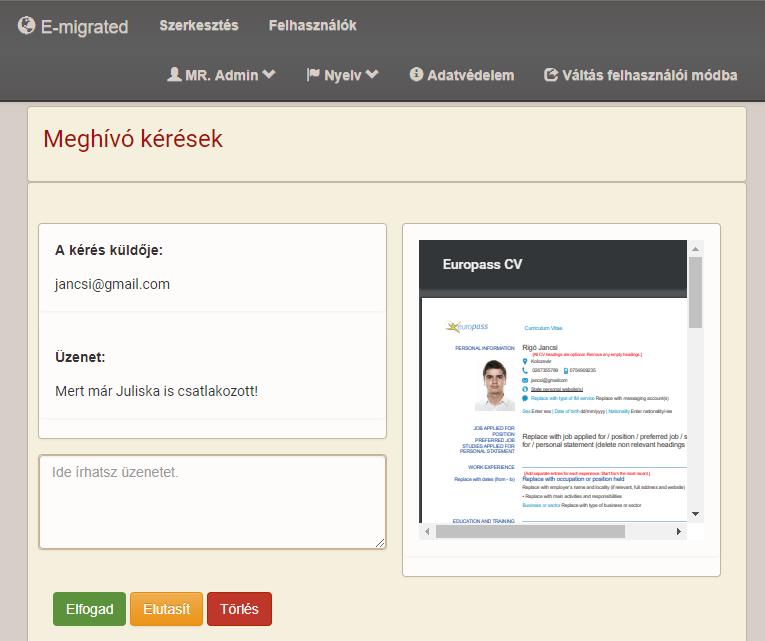
\includegraphics[width=0.9\linewidth]{images/meghivo_keres_admin}
    \end{minipage}
    \begin{minipage}{0.49\linewidth}
        \centering
        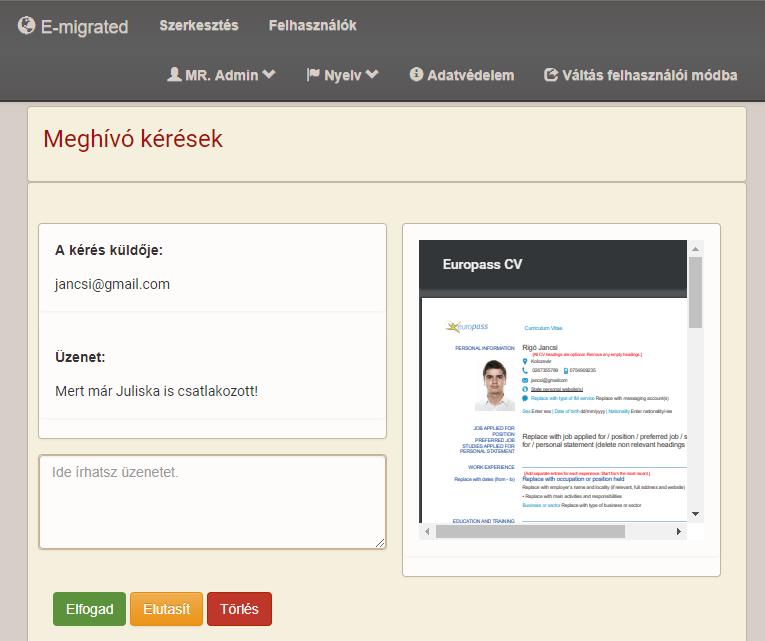
\includegraphics[width=0.9\linewidth]{images/meghivo_keres_admin}
    \end{minipage}
    \caption{A bal oldali képen láthatóak a beérkezett meghívó kérések, amelyeket az adminisztrátorok egy rövid üzenet kíséretében elfogadhatnak, elutasíthatnak vagy törölhetnek. A jobb oldali képen láthatóak az adminisztrátor által kilistázott felhasználók, itt függeszthetik fel a felhasználókat és kereshetnek közöttük név szerint. }
    \label{fig:admin}
\end{figure}













\chapter{Következtetések és továbbfejlesztési lehetőségek}
\label{ch:kovetkeztetes}

Az E-migrated alkalmazás célja egy olyan közösség kialakítása, melynek tagjai Székelyföldről elszármazott, vagy ott élő szakemberek, akik támogatják és segítik egymást, megosztják tapasztalataikat, tudásukat másokkal, ezáltal hozzájárulva a régió technológiai és gazdasági fejlődéséhez. 

A kezdeti nehézségek ellenére sikerült az alapötletnek megfelelő, működő prototípust létrehozni, mely alapjául szolgálhat egy későbbi, éles projektnek is, hiszen a fejlesztés során mindvégig fontos szempont volt az egyszerű bővíthetőség, újrafelhasználhatóság és tesztelhetőség.  A korán kialakított, szilárd alapokon álló architektúrának és az átgondolt design döntéseknek köszönhetően ezt sikerült is megvalósítani. 

A projekt fejlesztése során a funkcionalitások listája folyamatosan bővült és változott. A Scrum munkamódszer alkalmazásából adódóan nem okozott gondot, hogy a projekt indulásakor nem állt rendelkezésre egy kidolgozott specifikáció, hiszen a fokozatosan érkező követelményeket, változásokat gördülékenyen sikerült kezelni. 

Az alkalmazás többszöri bemutatása során a hallgatóságtól érkező visszajelzések és kérdések alapján nagyon sok továbbfejlesztési lehetőség fogalmazódott meg. Ilyen például a bejegyzések téma szerinti rendezése; különböző oktató anyagok, videók közzétételének megvalósítása; teljes, szöveg alapú keresés profiladatok alapján; más szociális hálók Google+, LinkedIn integrálása és a felhasználók egymás közötti kommunikációjának biztosítása. Továbbá felmerült az ötlete egy \textit{gamification} eszköz bevezetésének, amely ösztönözné a felhasználókat, hogy egymáson segítsenek, hiszen a segítségért KÖSZI pontokat kaphatnának, illetve adhatnának, ezáltal nyilvános elismerésben részesítve a jó szándékú személyt. A megszerzett KÖSZI pontok kiváltságokhoz vezethetnének gazdájuk számára, például további meghívókat kaphatnának. 

Végeredményként megfogalmazható, hogy egy alaposan megtervezett és gondosan formált webes alkalmazást sikerült létrehozni, amely hozzájárulhat egy digitális közösség kialakításához, annak fenntartásához, illetve Székelyföld regionális, technológiai és gazdasági fejlődéséhez. Összekapcsolja az egymástól, otthonuktól elszakadt szakembereket, lehetőséget teremtve számukra a szakmai tapasztalatcserére, segítségkérésre és -nyújtásra, valamint az itthon tevékenykedő szakemberekkel való kapcsolatfelvételre, amely potenciálisan hozzájárulhat az emigrált felhasználók hazaköltözéséhez. 


\appendix
\include{programok}


{ \renewcommand{\baselinestretch}{0.8}
  \normalsize 
  \setlength{\itemsep}{-2.4mm}
  \setlength{\bibspacing}{0.67\baselineskip}
  \bibliographystyle{abbrvnat_hu}
  \bibliography{dolgozat}
}

\end{document}
